The high-level motivation of GCN-SA
is to combine three sources 
of information for learning by the downstream GCN:
node feature information,
short-range, and long range structural information
We focus on the long-range structure learning by
\textsc{GCN-SA}'s utilization of SA
with \emph{reconnected adjacency matrix generation}.

\begin{figure}
  \centering
  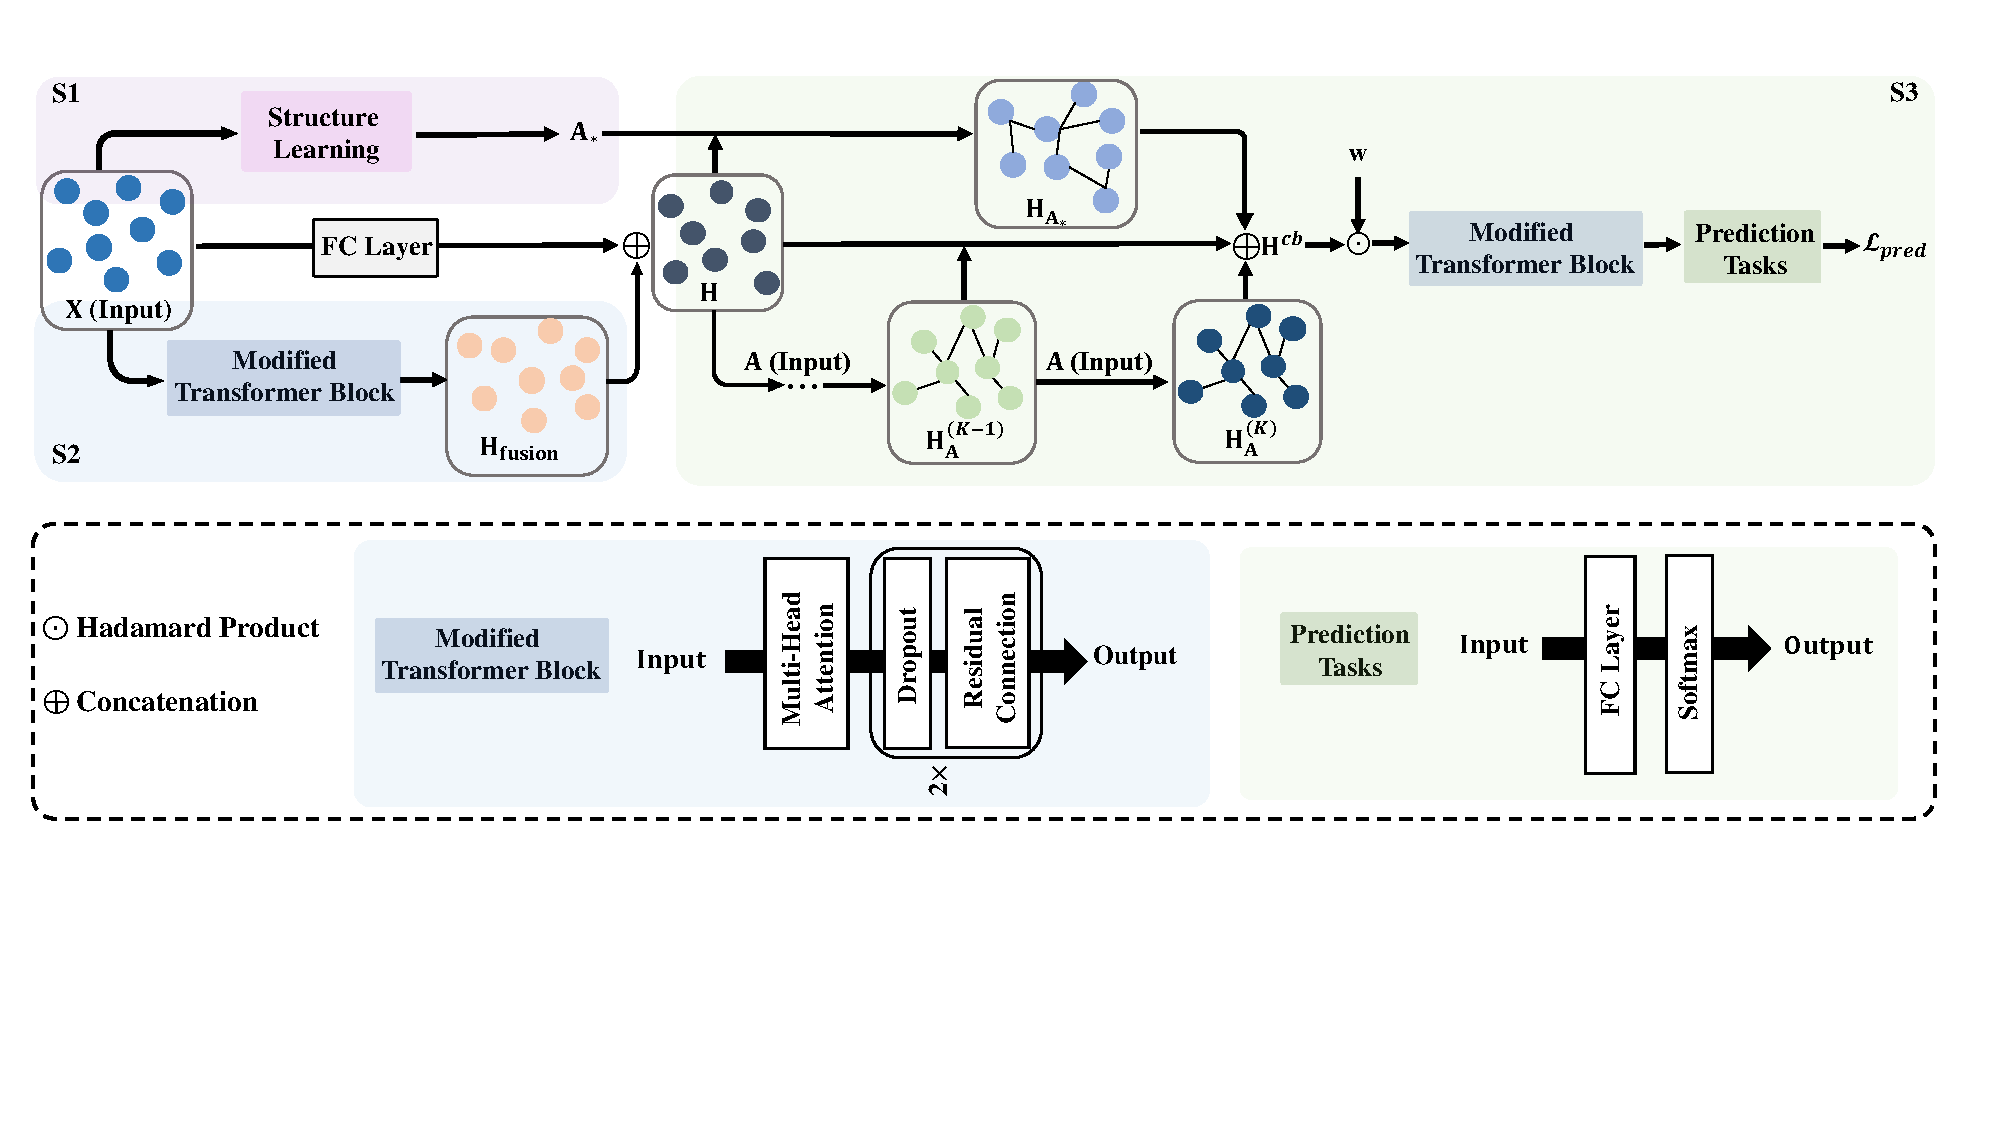
\includegraphics[page=1, width=\linewidth]{src/flowchart.pdf}
  \label{fig:flowchart}
  \caption{\textsc{GCN-SA} architecture
  \citep{jiang2024self}.}
\end{figure}

% \subsubsection{Reconnected Adjacency Matrix}

The motivation for learning a reconnected adjacency matrix
is to represent long-range connections between nodes.
An attention score matrix 
$ \mathbf{S} \in \mathbb{R}^{n\times n}$
is formed to generate a sparse reconnected adjacency matrix
$ \mathbf{A}^* \in \mathbb{R}^{n\times n}$
via $ H $-headed multi-head self-attention (MHSA):
\begin{flalign}
  \mathbf{S}
  &= \frac{1}{H} \sum_{h=1}^{H}
  \textrm{cosine}(\mathbf{X}\mathbf{W}_h^{Q}),
\end{flalign}

where $ \mathbf{W}_h^{Q} \in \mathbb{R}^{d\times p}  $
are learnable parameters corresponding to head
$ h = 1, \cdots, H $,
$ \textrm{cosine}\colon 
\mathbb{R}^{n \times p} \to [-1, 1]^{n \times n} $ 
the pairwise cosine similarity function for matrix
columns,
and $ \mathbf{S} \in [-1, 1]^{n \times n} $ the attention score matrix.
Once $ \mathbf{S} $ is obtained,
we construct the reconnected adjacency matrix
$ \mathbf{A}^* \in \left\{ 0, 1 \right\}^{n\times n} $
with a combined
$ k $NN and minimum-threshold approach:
\begin{flalign*}
  A^*_{ij} = \mathbbm{1} \left\{ 
    S_{ij} > \varepsilon \text{ or } S_{ij} \in R_i
  \right\}
\end{flalign*}

for hyperparameters $ \varepsilon, r $
and $ R_i $ denotes the $ r $ largest elements
of row $ S_{i\cdot} $.
A minor point is afterwards we set 
$ A^*_{ij} = \max \left\{ A^*_{ij}, A^*_{ji} \right\}$
to enforce symmetry.
The intention of this procedure 
is to ensure $ \mathbf{A}^* $ is \emph{sparse}
for better downstream performance \citep{jiang2024self}.
More specifically, each node attends to
$ \mathcal{O}(1) $ other nodes.
We touch on this in subsection 2.4.
For simplicity the authors denote
\begin{flalign*}
  \mathbf{A}^*
  &= \textrm{StructureLearning}(\mathbf{X}; \mathbf{W}^Q).
\end{flalign*}

parameterized by 
query parameters 
$ \mathbf{W}^Q = (
  \mathbf{W}^Q_1,
  \cdots, 
  \mathbf{W}^Q_H
) $.
Once $ \mathbf{A}^* $ is computed,
it is used downstream to compute
$ \mathbf{H}_{\mathbf{A}^*} $, 
representing aggregated long-range information:
\begin{flalign*}
  \mathbf{H}_{\mathbf{A}^{*}}
  = \mathbf{D}_*^{- \frac{1}{2}}
    \mathbf{A}^{*}
    \mathbf{D}_*^{- \frac{1}{2}}
    \mathbf{H}
\end{flalign*}

for $ \mathbf{D}_* = \text{diag}(\mathbf{A}^* \mathbf{1}_n) $ 
the degree matrix of $ \mathbf{A}^* $
and $ \mathbf{H} \in \mathbb{R}^{n \times q} $
representing node embeddings with hidden dimension $ q $.
% \mathbf{H}_\mathbf{A}^{*} 
% = \textrm{Fuse}(\mathbf{A}^{*}, \mathbf{H})
% \in \mathbb{R}^{n\times d}
% $. 
% Details on Fuse are included in the appendix.

% \subsubsection{Modified Transformer Block}

% Stages 2 and 3 of \textsc{GCN-SA} utilize a 
% transformer block:
% a fully-connected layer 
% followed by a self-attention layer.
% To mitigate overfitting
% (an issue prone to GCNs \citep{jiang2024self}),
% self-attention is followed by residual connection and dropout.
% The query parameters $ \mathbf{W}^Q $ are re-used
% in the transformer.
% We denote
% \begin{flalign*}
%   \mathbf{H} = \textrm{ModifiedTransformerBlock}(
%     \mathbf{X};
%     \mathbf{W}^Q,
%     \mathbf{W}^K,
%     \mathbf{W}^V,
%     \mathbf{W}^0
% )
% \end{flalign*}

% parameterized by the query, key, value,
% and fully-connected parameters.
% More detailed mathematical description
% can be seen is the appendix.

% \subsubsection{Feature Aggregation}

% Stepping back a little,
% GCN-SA utilize the reconnected adjacency
% matrix and the modified transformer blocks
% for feature aggregation in the following
% key sections of computation:
% \begin{enumerate}
%   \item Reconnected matrix formed from node features:
%     $ \mathbf{A}^* = \textrm{StructureLearning}(\mathbf{X}) $,
%   \item Feature embeddings 
%     $ \mathbf{H} \in \mathbb{R}^{n \times q} $ are formed 
%     from transformer block:
%     $ \mathbf{H} 
%     = \textrm{ModifiedTransformerBlock}(\mathbf{X}) $
%   \item $ \mathbf{H}_\mathbf{A}^{(k-1)},
%     \mathbf{H}_\mathbf{A}^{(k)} \in \mathbb{R}^{n \times q}$,
%     representing short-range structural information of $ G $,
%     are computed as:
%     $ \mathbf{H}_\mathbf{A}^{(k)} 
%     = \textrm{Fuse}(\mathbf{A}, \mathbf{H}_\mathbf{A}^{(k)}) $
%     for hyperparameter $ k $
%     and feature fusion function $ \textrm{Fuse} $.
%     Details on Fuse are included in the appendix.
%   \item $ \mathbf{H}^{cb} $, representing the combined information
%     of node features, short-range, and long-range structural
%     information,
%     is formed by concatenation:
%     \begin{flalign*}
%       \mathbf{H}^{cb} = \begin{bmatrix}
%         \mathbf{H}_\mathbf{A}^{(k-1)} &  
%         \mathbf{H}_\mathbf{A}^{(k)} &
%         \mathbf{H}_\mathbf{A}^{*} &
%         \mathbf{H}
%       \end{bmatrix}
%       \in \mathbb{R}^{n \times 4q}.
%     \end{flalign*}
% \end{enumerate}
